%----------------------------------------------------------------------------------------
%    PACKAGES AND THEMES
%----------------------------------------------------------------------------------------

\documentclass[xcolor=dvipsnames]{beamer}
\usetheme{SimpleDarkBlue}

\usepackage{hyperref}
\usepackage{graphicx}
\usepackage{booktabs}
\usepackage[spanish]{babel}
\usepackage[utf8]{inputenc}
\usepackage{amsmath}
\usepackage{amssymb}
\usepackage{amsthm}
\usepackage{graphics}
\usepackage{subfigure}
\usepackage{lipsum}
\usepackage{array}
\usepackage{multicol}
\usepackage{enumerate}
\usepackage[framemethod=TikZ]{mdframed}
\usepackage{geometry}
\usepackage{tikz}
\usepackage{pgffor}
\usepackage{ifthen}
\usepackage{enumitem}
\usepackage{hyperref}
\usepackage{listings}
\usepackage{bbm}

%Gestión de Hipervínculos

\hypersetup{
    colorlinks=true,
    linkcolor=black,
    filecolor=magenta,      
    urlcolor=cyan
}

%En esta parte se hacen redefiniciones de algunos comandos para que resulte agradable el verlos%

\def\proof{Demostración:\\}
\def\endproof{\hfill$\blacksquare$}

\def\sol{Solución:\\}
\def\endsol{\hfill$\square$}

%En esta parte se definen los comandos a usar dentro del documento para enlistar%

\newtheoremstyle{largebreak}
  {}% use the default space above
  {}% use the default space below
  {\normalfont}% body font
  {}% indent (0pt)
  {\bfseries}% header font
  {}% punctuation
  {\newline}% break after header
  {}% header spec

\theoremstyle{largebreak}

\newmdtheoremenv[
    hidealllines = true
]{exa}{Ejemplo}[section]

\newmdtheoremenv[
    hidealllines = true
]{obs}{Observación}[section]

\newmdtheoremenv[
    hidealllines = true
]{theor}{Teorema}[section]

\newmdtheoremenv[
    hidealllines = true
]{propo}{Proposición}[section]

\newmdtheoremenv[
    hidealllines = true
]{cor}{Corolario}[section]

\newmdtheoremenv[
    hidealllines = true
]{lema}{Lema}[section]

\newmdtheoremenv[
    hidealllines = true
]{mydef}{Definición}[section]

\newmdtheoremenv[
    hidealllines = true
]{excer}{Ejercicio}[section]

%En esta parte se colocan comandos que definen la forma en la que se van a escribir ciertas funciones%

\newcommand\abs[1]{\ensuremath{\left|#1\right|}}
\newcommand\divides{\ensuremath{\bigm|}}
\newcommand\cf[3]{\ensuremath{#1:#2\rightarrow#3}}
\newcommand\contradiction{\ensuremath{\#_c}}
\newcommand\natint[1]{\ensuremath{\left[\big|#1\big|\right]}}
\newcounter{figcount}
\setcounter{figcount}{1}
\newcommand{\bbm}[1]{\ensuremath{\mathbbm{#1}}}
\newcommand{\pint}[2]{\langle#1\big|#2 \rangle}
\newcommand{\norm}[1]{\|#1\|}
\newcommand{\Isom}[1]{\ensuremath{\textup{Isom}\left(#1\right)}}
\newcommand{\SO}[1]{\ensuremath{\textup{SO}\left(#1\right)}}
\newcommand\Aut[1]{\ensuremath{\textup{Aut}\left(#1\right)}}
\newcommand{\Cay}[1]{\ensuremath{\textup{Cay}\left(#1\right)}}
\newcommand{\gen}[1]{\ensuremath{\langle#1\rangle}}
\newcommand{\qisom}{\ensuremath{\underset{C.I.}{\sim}}}
\newcommand{\SL}[1]{\ensuremath{\textup{SL}\left(#1\right)}}
\newcommand{\PSL}[1]{\ensuremath{\textup{PSL}\left(#1\right)}}
\newcommand{\Tr}[1]{\ensuremath{\textup{Tr}\left(#1\right)}}
\newcommand{\im}[1]{\ensuremath{\textup{im}\left(#1\right)}}
\newcommand{\Diam}[1]{\ensuremath{\textup{diam}\left(#1\right)}}
\newcommand{\arcosh}[1]{\ensuremath{\textup{arcosh}\left(#1\right)}}

%----------------------------------------------------------------------------------------
%    TITLE PAGE
%----------------------------------------------------------------------------------------

\subtitle{Proyecto: Grupos y Geometría: Acciones, Dimensión y Dualidad}
\title{Plano Hiperbólico, Aplicaciones del Teorema de Svarc-Milnor y Grupos Hiperbólicos}

\author{Cristo Daniel Alvarado}

\institute
{
    Escuela Superior de Física y Matemáticas \\
    Instituto Politécnico Nacional
}
\date{\today} % Date, can be changed to a custom date

%----------------------------------------------------------------------------------------
%    PRESENTATION SLIDES
%----------------------------------------------------------------------------------------

\begin{document}

\begin{frame}
    \titlepage
\end{frame}

\begin{frame}{Index}
    \tableofcontents
\end{frame}

\section{El Plano Hiperbólico $\bbm{H}^2$ y su Grupo de Isometrías}

\subsection{El Grupo $\PSL{2,\bbm{R}}$}

\begin{frame}
    \begin{center}
        \Huge{El Plano Hiperbólico $\bbm{H}^2$ y su Grupo de Isometrías}
    \end{center}
    \begin{figure}
        \begin{center}
            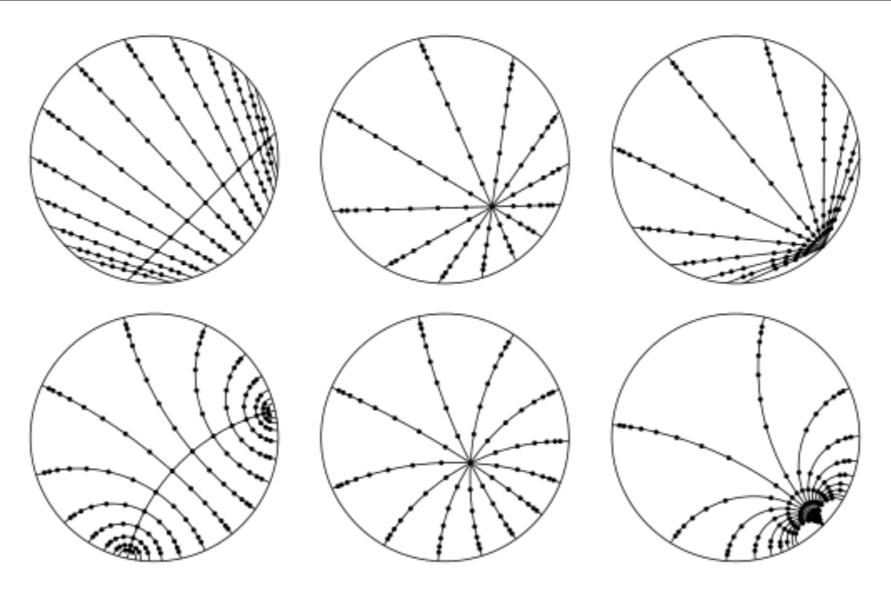
\includegraphics[scale=0.3]{images/isometries_2.png}
        \end{center}
    \end{figure}
\end{frame}

\begin{frame}
    \begin{center}
        \Large El Grupo $\PSL{2,\bbm{R}}$

        \hfill\break
        \pause
        \Huge$\PSL{2,\bbm{R}}\curvearrowright\bbm{H}^2$
    \end{center}
\end{frame}

\begin{frame}{El Grupo $\PSL{2,\bbm{R}}$}
    \begin{mydef}
        $\SL{n,\bbm{A}}$ denota al espacio de todas las matrices $n\times n$ con entradas en $\bbm{A}\subseteq\bbm{C}$ tales que:
        \begin{equation*}
            \det(A)=1,\quad\forall A\in\bbm{A}
        \end{equation*}
    \end{mydef}
\end{frame}

\begin{frame}{El Grupo $\PSL{2,\bbm{R}}$}
    \begin{mydef}[\textbf{Transformaciones de Möbius}]
        Para la matriz $2\times 2$:
        \begin{equation*}
            A=\left(
                \begin{array}{cc}
                    a & b \\
                    c & d \\
                \end{array}
             \right)\in\SL{2,\bbm{R}}
        \end{equation*}
        definimos la \textbf{transformación de Möbius asociada} $\cf{f_A}{H}{H}$, dada por:
        \begin{equation*}
            z\mapsto\frac{a\cdot z+b}{c\cdot z+d}
        \end{equation*}
    \end{mydef}
\end{frame}

\begin{frame}{El Grupo $\PSL{2,\bbm{R}}$}
    \begin{obs}
        Toda transformación de Möbius está bien definida, ya que como $H$ es el plano superior, entonces la parte real de $z$ nunca será un número con parte imaginaria cero, así que $c\cdot z+d\neq 0$ para todo $z\in H$.
    \end{obs}

    \begin{exa}
        La función $z\mapsto z$ es una transformación de Möbius. Al igual que la función $z\mapsto\frac{1}{z}$. En particular, todas las funciones lineales de $H$ en $H$ son transformaciones de Möbius.
    \end{exa}
\end{frame}

\begin{frame}{El Grupo $\PSL{2,\bbm{R}}$}
    \begin{propo}
        Se tiene lo siguiente:
        \begin{enumerate}[label = \textit{(\arabic*)}]
            \item $f_A$ está bien definido y es un difeomorfismo $C^\infty$ (o suave).
            \item Para todo $A,B\in\SL{2,\bbm{R}}$ se tiene que $f_{A\cdot B}=f_A\circ f_B$.
            \item $f_A=f_{-A}$ para todo $A\in\SL{2,\bbm{R}}$.
        \end{enumerate}
    \end{propo}

    \begin{proof}
        De \textit{(1)} y \textit{(2)}: Son inmediatas.

        De \textit{(3)}: Si
        \begin{equation*}
            A=\left(
                \begin{array}{cc}
                    a & b \\
                    c & d \\
                \end{array}
             \right)\in\SL{2,\bbm{R}}
        \end{equation*}
        entonces,
        \begin{equation*}
            f_A(z)=\frac{a\cdot z+b}{c\cdot z+d}=\frac{-a\cdot z+-b}{-c\cdot z+-d}=f_{-A}(z)
        \end{equation*}
        para todo $z\in H$.
    \end{proof}

\end{frame}


\begin{frame}{El Grupo $\PSL{2,\bbm{R}}$}
    \begin{exa}[\textbf{Generadores $\SL{2,\bbm{R}}$}]
        Tenemos los siguientes dos tipos de transformaciones de Möbius:
        \begin{itemize}
            \item Sea $b\in\bbm{R}$. Entonces, la transformación de Möbius asociada a la matriz:
            \begin{equation*}
                \left(\begin{array}{cc}
                    1 & b \\
                    0 & 1 \\
                \end{array} \right)\in\SL{2,\bbm{R}}
            \end{equation*}
            es la traslación horizontal $z\mapsto z+b$ en $H$ por un factor $b$ se denotará por $T_b$.
            \item La transformación de Möbius asociada a la matriz:
            \begin{equation*}
                \left(\begin{array}{cc}
                    0 & 1 \\
                    -1 & 0 \\
                \end{array} \right)\in\SL{2,\bbm{R}}
            \end{equation*}
            es la función $z\mapsto-\frac{1}{z}$ se denotará por $-In$.
        \end{itemize}
    \end{exa}
\end{frame}

\begin{frame}{El Grupo $\PSL{2,\bbm{R}}$}
    \begin{exa}[\textbf{Generadores $\SL{2,\bbm{R}}$}]
        Se tiene que el grupo $\SL{2,\bbm{R}}$ es generado por:
        \begin{equation*}
            \left\{\left(\begin{array}{cc}
                0 & 1 \\
                -1 & 0 \\
            \end{array} \right)\right\}\cup\left\{\left(\begin{array}{cc}
                1 & b \\
                0 & 1 \\
            \end{array} \right)\Big|b\in\bbm{R} \right\}
        \end{equation*}
    \end{exa}
\end{frame}

\begin{frame}{El Grupo $\PSL{2,\bbm{R}}$}
    \begin{propo}[\textbf{Transformaciones de Möbius son isometrías}]
        Si $A\in\SL{2,\bbm{R}}$, entonces la transformación de Möbius asociada $\cf{f_A}{H}{H}$ es una isometría Riemanniana de $\bbm{H}^2$. En particular, tenemos un monomorfismo de grupos:
        \begin{equation*}
            \PSL{2,\bbm{R}}=\SL{2,\bbm{R}}/\left\{I,-I \right\}\rightarrow\Isom{H,d_H}
        \end{equation*}
        dado por $[A]\mapsto f_A$.
    \end{propo}

    \begin{proof}
        Por el ejemplo anterior basta con ver que $T_b$ y $In$ son isometrías Riemannianas de $\bbm{H}^2$, ya que la composición de isometrías Riemannianias sigue siendo una isometría Riemanniana.
    \end{proof}
\end{frame}

\begin{frame}{El Grupo $\PSL{2,\bbm{R}}$}
    \begin{theor}[\textbf{El grupo de isometrías hiperbólicas}]
        El grupo $\Isom{H,d_H}$ es generado por:
        \begin{equation*}
            \left\{f_A\Big|A\in\SL{2,\bbm{R}} \right\}\cup\left\{z\mapsto-\overline{z} \right\}
        \end{equation*}
        En particular, toda isometría de $(H,d_H)$ es una isometría Riemanniana suave y, $\Isom{H,d_H}=\Isom{\bbm{H}^2}$. Además, la función:
        \begin{equation*}
            \begin{split}
                \PSL{2,\bbm{R}}&\rightarrow\Isom{H,d_H}^+\\
                [A]&\mapsto f_A\\
            \end{split}
        \end{equation*}
        es un isomorfismo, siendo $\Isom{H,d_H}^+$ al grupo de todas las isometrías que preservan orientación de $\Isom{H,d_H}$.
    \end{theor}
\end{frame}

\subsection{Acción de $\SL{2,\bbm{R}}$ en $\bbm{H}^2$}

\begin{frame}
    \begin{center}
        \Large Acción de $\SL{2,\bbm{R}}$ en $\bbm{H}^2$
    \end{center}
\end{frame}

\begin{frame}{Acción de $\SL{2,\bbm{R}}$ en $\bbm{H}^2$}
    \begin{propo}[\textbf{Acción de $\SL{2,\bbm{R}}$ en $H$}]
        \label{accionSL2RenH}
        La acción de $\SL{2,\bbm{R}}$ en $H$:
        \begin{equation*}
            \cf{f}{\SL{2,\bbm{R}}}{\textup{Sym}(H)}
        \end{equation*}
        tal que $A\mapsto f_A$ cumple lo siguiente:
        \begin{enumerate}[label = \textit{(\arabic*)}]
            \item El grupo $\SL{2,\bbm{R}}$ actúa en $H$ vía transformaciones de Möbius, más aún, esta acción es transitiva.
            \item El subgrupo estabilizador de $i$ respecto a esta acción es $\SO{2}$.
            \item Para todo $z,z'\in H$ existe $A\in\SL{2,\bbm{R}}$ tal que:
            \begin{equation*}
                f_A(z)=i\quad\textup{y}\quad\Re(f_A(z'))=0, \Im(f_A(z'))>1
            \end{equation*}
        \end{enumerate}
    \end{propo}
\end{frame}

\begin{frame}{Acción de $\SL{2,\bbm{R}}$ en $\bbm{H}^2$}
    \textit{Demostración}:

    De \textit{(1)}: Es inmediato que el grupo actúa via transformaciones de Möbius con la acción dada por:
    \begin{equation*}
        (A,z)\mapsto A\cdot z = f_A(z),\quad\forall A\in \SL{2,\bbm{R}},\forall z\in H
    \end{equation*}
    Veamos que esta acción es transitiva. Basta probar que para todo $z\in H$ existe un $A_z\in\SL{2,\bbm{R}}$ tal que:
    \begin{equation*}
        f_{A_z}(z)=i
    \end{equation*}
    Tomemos $x=\Re(z)$ y $y=\Im(z)$. Entonces la transformación de Möbius asociada a la matriz:
    \begin{equation*}
        A_z=\left(
            \begin{array}{cc}
                \frac{1}{\sqrt{y}} & -\frac{x}{\sqrt{y}} \\
                0 & \sqrt{y} \\
            \end{array}
        \right)\in\SL{2,\bbm{R}}
    \end{equation*}
    es tal que:
    \begin{equation*}
        A_z\cdot z=f_{ A_z}(z)=\frac{\frac{x+iy}{\sqrt{y}}-\frac{x}{\sqrt{y}}}{\sqrt{y}}=i
    \end{equation*}
\end{frame}

\begin{frame}{Acción de $\SL{2,\bbm{R}}$ en $\bbm{H}^2$}
    Con lo que la acción es transitiva.
    
    De \textit{(2)}: Se tiene que:
    \begin{equation*}
        \begin{split}
            \SL{2,\bbm{R}}_i&=\left\{A\in\SL{2,\bbm{R}}\Big|A\cdot i=i \right\}\\
            &=\left\{\left(\begin{array}{cc}
                a & b \\
                c & d \\
            \end{array} \right) \in\SL{2,\bbm{R}}\Big|a = d\textup{ y }c=-b \right\}\\
            &=\left\{\left(\begin{array}{cc}
                a & -c \\
                c & a \\
            \end{array} \right) \in\mathcal{M}_{2\times2}(\bbm{R}) \Big|a^2+c^2=1 \right\}\\
            &=\SO{2}\\
        \end{split}
    \end{equation*}

    De \textit{(3)}: Inmediato del inciso \textit{(1)}.
\end{frame}

\begin{frame}{Acción de $\SL{2,\bbm{R}}$ en $\bbm{H}^2$}
    Resulta que podemos dotar al grupo $\PSL{2,\bbm{R}}$ con una topología. Para ello, notemos que la función:
    \begin{equation*}
        [A]\mapsto (a,b,c,d)
    \end{equation*}
    es una función suprayectiva de $\PSL{2,\bbm{R}}$ en el subconjunto:
    \begin{equation*}
        \left\{(a,b,c,d)\in\bbm{R}^4\Big|ad-bc=1 \right\}
    \end{equation*}
    y es una función biyectiva al espacio cociente:
    \begin{equation*}
        \left\{(a,b,c,d)\in\bbm{R}^4\Big|ad-bc=1 \right\}/\left\{(a,b,c,d)\sim(-a,-b,-c,-d) \right\}
    \end{equation*}
\end{frame}

\begin{frame}{Acción de $\SL{2,\bbm{R}}$ en $\bbm{H}^2$}
    Dotando al subespacio $\left\{(a,b,c,d)\in\bbm{R}^4\Big|ad-bc=1 \right\}$ con la norma usual de $\bbm{R}^4$ resulta que el cociente también se puede dotar de una norma, así que el grupo $\PSL{2,\bbm{R}}$ tiene una norma inducida por la norma del espacio cociente, a saber:
    \begin{equation*}
        \norm{[A]}=\sqrt{a^2+b^2+c^2+d^2}
    \end{equation*}
    donde
    \begin{equation*}
        A=\left(\begin{array}{cc}
            a & b \\
            c & d \\
        \end{array}\right)
    \end{equation*}
\end{frame}

\begin{frame}{Acción de $\SL{2,\bbm{R}}$ en $\bbm{H}^2$}
    \begin{propo}
        $\PSL{2,\bbm{R}}$ es un grupo topológico con la métrica inducida por la norma:
        \begin{equation*}
            \norm{[A]}=\sqrt{a^2+b^2+c^2+d^2}
        \end{equation*}
    \end{propo}
\end{frame}

\subsection{Švarc-Milnor y el plano hiperbólico}

\begin{frame}
    \begin{center}
        \Large Švarc-Milnor y el plano hiperbólico
    \end{center}
\end{frame}

\begin{frame}{Švarc-Milnor y el plano hiperbólico}
    \begin{lema}[\textbf{Švarc-Milnor}]
        Sea $G$ un grupo actuando en un espacio métrico no vacío $(X,d)$ por isometrías. Suponga que existen constantes $c,b\in\bbm{R}_{>0}$ tales que $(X,d)$ es $(c,d)$-cuasi-geodésico y además que existe un conjunto $B\subseteq X$ con las siguientes propiedades:
        \begin{itemize}
            \item El diámetro de $B$ es finito.
            \item Las traslaciones de $B$ cubren a todo $X$, esto es: $\bigcup_{g\in G}g\cdot B=X$.
            \item El conjunto $S=\left\{g\in G\Big|g\cdot B'\cap B'\neq\emptyset \right\}$ es finito, donde:
            \begin{equation*}
                B'=B_{2\cdot b}^{(X,d)}(B)=\left\{x\in X\Big|\exists y\in B\textup{ tal que }d(x,y)\leq 2b \right\}
            \end{equation*}
        \end{itemize}
    \end{lema}
\end{frame}

\begin{frame}{Švarc-Milnor y el plano hiperbólico}
    \begin{lema}[\textbf{Švarc-Milnor}]
        Entonces:
        \begin{enumerate}[label = \textit{(\arabic*)}]
            \item El grupo $G$ es generado por $S$; en particular, $G$ es finitamente generado.
            \item Para todo $x\in X$, la función:
            \begin{equation*}
                \begin{split}
                    G&\rightarrow X\\
                    g&\mapsto g\cdot x\\
                \end{split}
            \end{equation*}
            es una cuasi-isometría (con respecto a la métrica de palabras en $G$). Por tanto, $G\qisom X$.
        \end{enumerate}
    \end{lema}
\end{frame}

\begin{frame}{Švarc-Milnor y el plano hiperbólico}
    \begin{obs}
        Notemos que para la acción de $\SL{2,\bbm{R}}$ en el espacio métrico $(H,d_H)$ estamos en la posibilidad de aplicar el lema anterior, solo basta verificar algunas condiciones. Las que ya se tienen son las siguientes:
        \begin{enumerate}[label = \textit{(\arabic*)}]
            \item El espacio $(H,d_H)$ es no vacío $(1,0)$-cuasi-geodésico, por ser geodésico.
            \item $\SL{2,\bbm{R}}$ actúa por isometrías en $(H,d_H)$.
        \end{enumerate}
        Para aplicar el lema, debemos ver que las tres condiciones del lema se cumplen para un conjunto $B\subseteq H$.
    \end{obs}
\end{frame}

\begin{frame}{Švarc-Milnor y el plano hiperbólico}
    Sea $B=\left\{z\right\}\subseteq H$. Se tiene que:
    \begin{enumerate}[label = \textit{(\arabic*)}]
        \item El diámetro de $B$ es cero, es decir que es finito.
        \item $\bigcup_{A\in\SL{2,\bbm{R}}}A\cdot B=\bigcup_{A\in\SL{2,\bbm{R}}}A\cdot\left\{z\right\}=H$, pues la acción de $\SL{2,\bbm{R}}$ en $H$ es transitiva.
        \item Como el espacio es $(1,0)$-cuasi-geodésico, solo hay que ver si el conjunto:
        \begin{equation*}
            \left\{A\cdot B\cap B\neq\emptyset \Big|A\in\SL{2,\bbm{R}} \right\}=\left\{A\cdot z=z\Big|A\in\SL{2,\bbm{R}} \right\}
        \end{equation*}
        es finito o no. Esto ya que en este caso se tiene:
        \begin{equation*}
            B'=B_{2\cdot 0}^{(X,d)}(B)=\left\{x\in X\Big|d(x,z)=0\right\}=B
        \end{equation*}
    \end{enumerate}
\end{frame}

\begin{frame}{Švarc-Milnor y el plano hiperbólico}
    Resulta que tal conjunto no es finito, pues si $A_z\in\SL{2,\bbm{R}}$ es tal que:
    \begin{equation*}
        f_{A_z}(z)=i
    \end{equation*}
    se tiene que:
    \begin{equation*}
        A_z^{-1}\cdot\SO{2}\cdot A_z\subseteq\left\{A\cdot B\cap B\neq\emptyset \Big|A\in\SL{2,\bbm{R}} \right\}
    \end{equation*}
    pues:
    \begin{equation*}
        f_{A_z^{-1}\cdot O\cdot A_z}(z)=f_{A_z^{-1}}\circ f_{O}\circ f_{A_z}(z)=f_{A_z^{-1}}\circ f_{O}(i)=f_{A_z^{-1}}(i)=z
    \end{equation*}
    con lo que el conjunto de la derecha no es finito, pues $A_z^{-1}\cdot\SO{2}\cdot A_z$ no lo es.
\end{frame}

\begin{frame}{Švarc-Milnor y el plano hiperbólico}
    \begin{center}
        \Large \textit{¿Cómo solucionamos este problema?}\\
        \pause
        \Large Usando subgrupos de $\SL{2,\bbm{R}}$ o equivalentemente de $\PSL{2,\bbm{R}}$.
    \end{center}
\end{frame}

%TODO: Seguir con Grupos Fuchsianos

\subsection{Grupos Fuchsianos}

\begin{frame}
    \begin{center}
        \Large Grupos Fuchsianos
    \end{center}
\end{frame}

\begin{frame}{Grupos Fuchsianos}
    \begin{cor}[\textbf{Formulación topológica del lema de Švarc-Milnor}]
        Sea $G$ un grupo actuando por isometrías en un espacio métrico no vacío $(X,d)$ propio y geodésico. Más aún, suponga que esta acción es propia y cocompacta. Entonces, $G$ es finitamente generado y, para todo $x\in X$ la función:
        \begin{equation*}
            \begin{split}
                G&\rightarrow X\\
                g&\mapsto g\cdot x\\
            \end{split}
        \end{equation*}
        es una cuasi-isometría.
    \end{cor}
\end{frame}

\begin{frame}{Grupos Fuchsianos}
    \begin{mydef}[\textbf{Familias localmente finitas}]
        Una familia $\left\{F_i\subseteq X\Big|i\in I \right\}$ de subconjuntos un espacio métrico $(X,d)$ es \textbf{localmente finita} si el conjunto:
        \begin{equation*}
            \left\{i\in I \Big|F_i\cap C\neq\emptyset \right\}
        \end{equation*}
        es un conjunto finito para todo $C\subseteq X$ compacto.
    \end{mydef}

    \begin{mydef}[\textbf{Acciones propias}]
        Decimos que un grupo $G$ actuando en un espacio métrico $(X,d)$ \textbf{actúa propiamente} si la familia $\left\{G\cdot x\Big|x\in X \right\}$ es localmente finita.

        En este caso diremos que la acción es \textbf{propia}.
    \end{mydef}
\end{frame}

\begin{frame}{Grupos Fuchsianos}
    \begin{mydef}[\textbf{Acciones cocompactas}]
        Una acción de un grupo $G$ en un espacio topológico $X$ es \textbf{cocompacta} si el espacio cociente $G/X$ es compacto respecto a la topología cociente.
    \end{mydef}
\end{frame}

\begin{frame}{Grupos Fuchsianos}
    \begin{mydef}
        Un subgrupo $H<\Isom{H,d_H}^+$ es llamado \textbf{discreto} si el grupo $H$ visto como subgrupo de $\PSL{2,\bbm{R}}$ es discreto.
        
        En tal caso, $H$ es llamado \textbf{grupo Fuchsiano}.
    \end{mydef}
\end{frame}

\begin{frame}{Grupos Fuchsianos}
    \begin{exa}
        El \textbf{grupo modular} $\PSL{2,\bbm{Z}}$ es un subgrupo discreto de $\PSL{2,\bbm{R}}$, por lo que es Fuchsiano.
    \end{exa}

    \begin{exa}
        El grupo $\PSL{2,\bbm{Q}}$ es un subgrupo de $\PSL{2,\bbm{R}}$ que no es discreto, luego no es Fuchsiano.
    \end{exa}
\end{frame}

\begin{frame}{Grupos Fuchsianos}
    \begin{exa}
        El conjunto de todas las traslaciones reales enteras $\left\{T_n\Big|n\in\bbm{Z} \right\}$ es un grupo Fuchsiano.
    \end{exa}

    \begin{exa}
        El conjunto de todas las traslaciones reales $\left\{T_r\Big|r\in\bbm{R} \right\}$ no es un grupo Fuchsiano por no ser discreto.
    \end{exa}
\end{frame}

\begin{frame}{Grupos Fuchsianos}
    \begin{theor}[\textbf{Caracterización de las acciones propias}]
        Un grupo $G$ actúa propiamente sobre un espacio métrico $(X,d)$ si y sólo si para todo $x\in X$ existe $\epsilon>0$ tal que:
        \begin{equation*}
            \left\{g\in G\Big|g\cdot B_\varepsilon^{(X,d)}(x)\cap B_\varepsilon^{(X,d)}(x)\neq\emptyset \right\}
        \end{equation*}
        es un conjunto finito.
    \end{theor}
\end{frame}

\begin{frame}{Grupos Fuchsianos}
    \begin{theor}[\textbf{Caracterización de los grupos Fuchsianos}]
        Sea $\Gamma<\PSL{2,\bbm{R}}$. Entonces, $\Gamma$ es Fuchsiano si y sólo si la acción es propia.
    \end{theor}
\end{frame}

\begin{frame}{Grupos Fuchsianos}
    \begin{theor}[\textbf{Cuasi-isometría de grupos Fuchsianos y $(H,d_H)$}]
        Sea $\Gamma<\PSL{2,\bbm{R}}$ un grupo Fuchsiano. Conisdere la acción de $\Gamma$ en $(H,d_H)$ dada por:
        \begin{equation*}
            [A]\mapsto f_A
        \end{equation*}
        Entonces, si la acción es cocompacta se sigue que $H\qisom \Gamma$ y, para todo $z\in H$ la función:
        \begin{equation*}
            [A]\mapsto [A]\cdot z=A\cdot z
        \end{equation*}
        es una cuasi-isometría.
    \end{theor}

    \pause

    \begin{proof}
        Inmediato del Corolario al lema de Svarc-Milnor y de la caracterización de los grupos Fuchsianos.
    \end{proof}
\end{frame}

%----------------------------------------------------------------------------------------
\section{Espacios Hiperbólicos}
%----------------------------------------------------------------------------------------

\begin{frame}{Espacios Hiperbólicos}
    \begin{center}
        \LARGE{Espacios Hiperbólicos}
    \end{center}

    \pause

    \begin{center}
        Hablaremos de triángulos.
    \end{center}
    \begin{figure}
        \begin{center}
            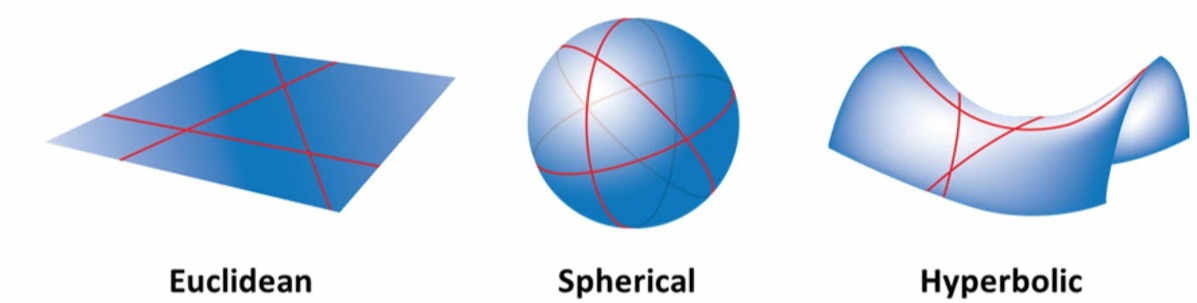
\includegraphics[scale=0.25]{images/all_triangles.png}
        \end{center}
    \end{figure}

\end{frame}

\begin{frame}{Hiperbólicidad y $\delta$-hiperbolicidad}
    \begin{center}
        Triángulos geodésicos sobre superficie \textit{hiperbólica}:
    \end{center}
    \begin{figure}
        \begin{center}
            
\includegraphics[scale=0.5]{images/hyperbolic_triangle_2.png}
        \end{center}
    \end{figure}
\end{frame}

\begin{frame}{Hiperbólicidad y $\delta$-hiperbolicidad}
    \textbf{Idea}: generalizar noción de hiperbolicidad a espacios métricos.
    \begin{itemize}
        \item Queremos conservar noción de distancia mínima (geodésicas).
        \item Vía triángulos geodésicos.
        \item Ensanchamientos.
    \end{itemize}

    \pause
    \begin{figure}
        \begin{center}
            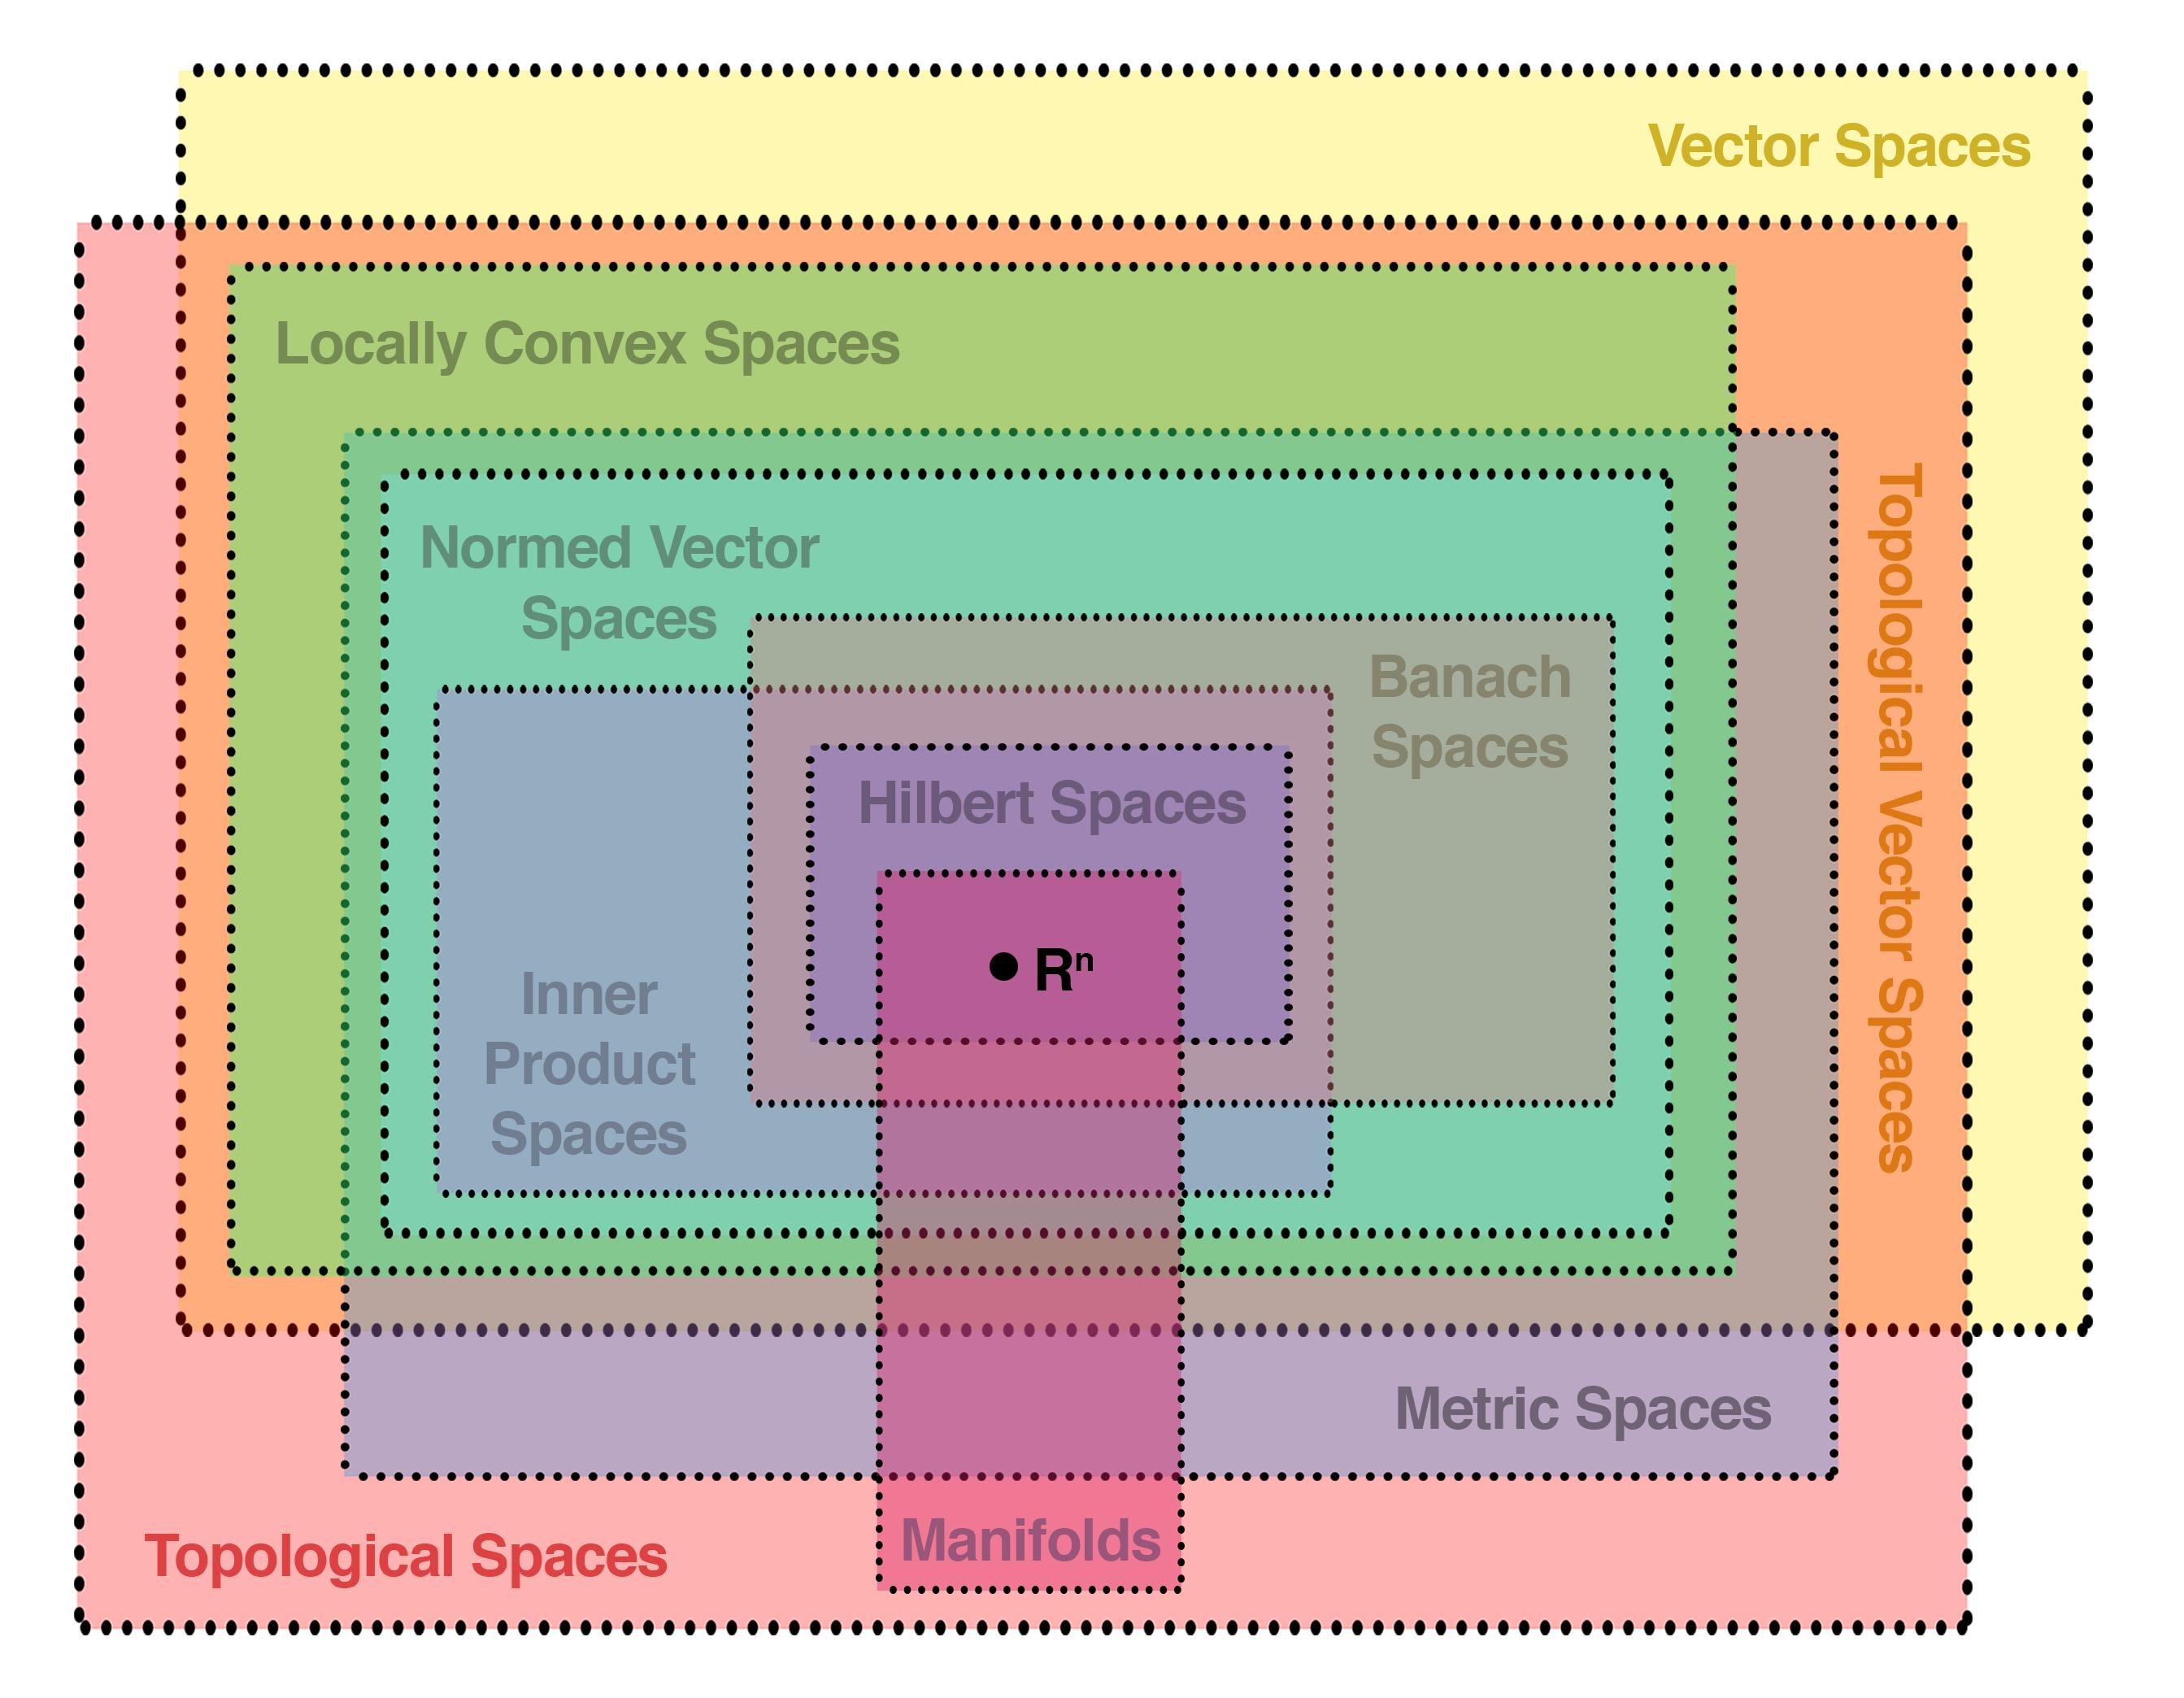
\includegraphics[scale=0.08]{images/hiearchy.jpg}
        \end{center}
    \end{figure}
\end{frame}

\begin{frame}{Hiperbólicidad y $\delta$-hiperbolicidad}
    \begin{center}
        Ensanchamiento:
    \end{center}
    \begin{figure}
        \begin{center}
            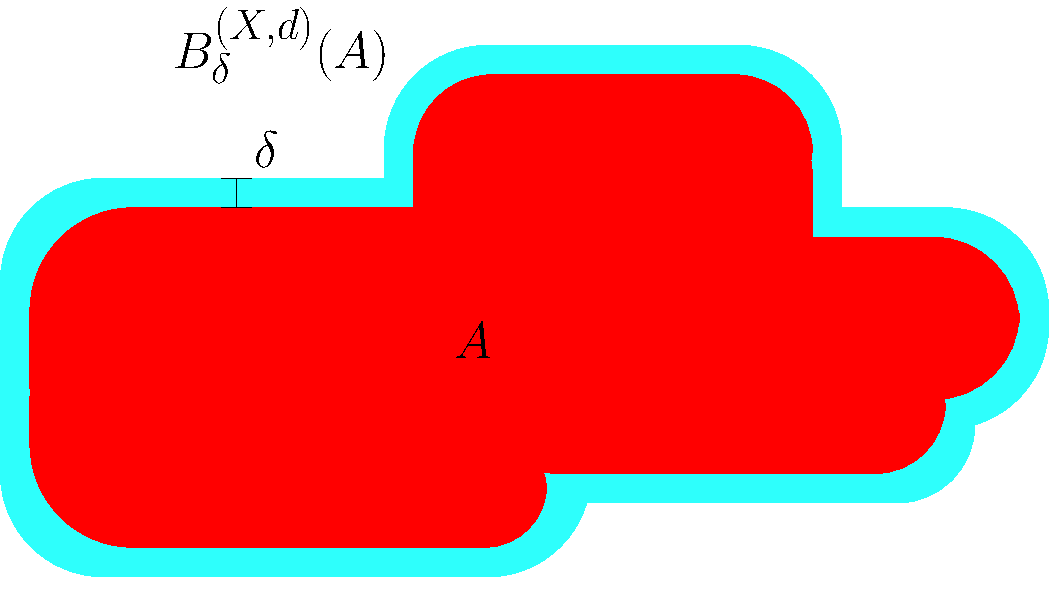
\includegraphics[scale=0.6]{images/B_delta.pdf}
        \end{center}
        \caption{Ejemplo de conjunto $A$ y $B_\delta^{(X,d)}(A)$ (ensanchamiento de $A$).}
    \end{figure}
\end{frame}

\begin{frame}{Hiperbólicidad y $\delta$-hiperbolicidad}
    \begin{mydef}
        Sea $(X,d)$ un espacio métrico. Para cada $\delta>0$ y para cada $A\subseteq X$ se define el conjunto:
        \begin{equation*}
            B_\delta^{(X,d)}(A)=\left\{x\in X\Big|\exists a\in A\textup{ tal que }d(x,a)\leq\delta \right\}
        \end{equation*}
        en este caso $B_\delta^{(X,d)}(A)$ será llamado \textbf{ensanchamiento de $A$ por factor $\delta$}.
    \end{mydef}
\end{frame}

\subsection{Hiperbólicidad y $\delta$-hiperbolicidad}

\begin{frame}{Hiperbólicidad y $\delta$-hiperbolicidad}
    \begin{figure}
        \begin{center}
            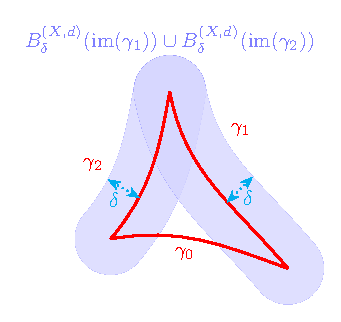
\includegraphics[scale=1.25]{images/delta_slim_2.pdf}
        \end{center}
        \caption{Triángulo geodésico $\Delta=(\gamma_0,\gamma_1,\gamma_2)$ y $B_\delta^{(X,d)}$.}
    \end{figure}
\end{frame}

\begin{frame}{Hiperbólicidad y $\delta$-hiperbolicidad}
    \begin{mydef}[\textbf{Triángulos geodésicos $\delta$-delgados}]
        Sea $(X,d)$ un espacio métrico. Un \textbf{triángulo geodésico en $X$} es una tripleta $(\gamma_0,\gamma_1,\gamma_2)$ de geodésicas $\cf{\gamma_i}{[0,L_i]}{X}$ en $X$ tales que:
        \begin{equation*}
            \gamma_0(L_0)=\gamma_1(0),\quad \gamma_1(L_1)=\gamma_2(0),\quad \gamma_2(L_2)=\gamma_0(0)
        \end{equation*}
    \end{mydef}

    \begin{mydef}[\textbf{Triángulos geodésicos $\delta$-delgados}]
        Un triángulo geodésico es \textbf{$\delta$-delgado} si:
        \begin{equation*}
            \begin{array}{cc}
                \im{\gamma_0}&\subseteq B_{\delta}^{(X,d)}(\im{\gamma_1}\cup\im{\gamma_2}),\\
                \im{\gamma_1}&\subseteq B_{\delta}^{(X,d)}(\im{\gamma_0}\cup\im{\gamma_2}),\\
                \im{\gamma_2}&\subseteq B_{\delta}^{(X,d)}(\im{\gamma_0}\cup\im{\gamma_1})
            \end{array}
        \end{equation*}
    \end{mydef}
\end{frame}

\begin{frame}{Hiperbólicidad y $\delta$-hiperbolicidad}
    \begin{center}
        \textit{\Large ¿El triángulo anterior es $\delta$-delgado?}
    \end{center}
    \pause
    \begin{center}
        \Large No, la imagen de $\gamma_0$ no está contenida en $B_\delta^{(X,d)}(\im{\gamma_1})\cup B_\delta^{(X,d)}(\im{\gamma_2})$.
    \end{center}
\end{frame}

\begin{frame}{Hiperbólicidad y $\delta$-hiperbolicidad}
    \begin{mydef}[\textbf{Espacios hiperbólicos}]
        Sea $(X,d)$ un espacio métrico.
        \begin{enumerate}[label = \textit{(\arabic*)}]
            \item Sea $\delta\in\bbm{R}_{\geq0}$. Decimos que $(X,d)$ es \textbf{$\delta$-hiperbólico} si $X$ es geodésico y todos los triángulos geodésicos de $X$ son $\delta$-delgados.
            \item $(X,d)$ es \textbf{hiperbólico} si existe $\delta\in\bbm{R}_{\geq0}$ tal que $(X,d)$ es $\delta$-hiperbólico.
        \end{enumerate}
    \end{mydef}

    \pause

    \begin{exa}
        Todo espacio métrico geodésico $X$ de diámetro finito es $\Diam{X}$-hiperbólico. 
    \end{exa}
\end{frame}

\begin{frame}{Hiperbólicidad y $\delta$-hiperbolicidad}
    \begin{exa}
        La recta real $\bbm{R}$ es $0$-hiperbólico ya que cada triángulo geodésico en $\bbm{R}$ es degenerado, pues estos se ven simplemente como líneas rectas.
    \end{exa}

    \pause

    \begin{exa}
        El plano euclideano $\bbm{R}^2$ no es hiperbólico.
    \end{exa}
\end{frame}

\begin{frame}{Hiperbólicidad y $\delta$-hiperbolicidad}
    \begin{figure}
        \begin{center}
            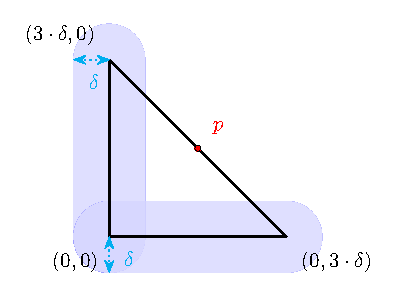
\includegraphics[scale=1.25]{images/hiperbolicnt_euclidean_plane.pdf}
        \end{center}
        \caption{$\bbm{R}^2$ no es hiperbólico.}
    \end{figure}
\end{frame}

\begin{frame}{Hiperbólicidad y $\delta$-hiperbolicidad}
    \begin{center}
        \Large\textit{¿Coincide esta nueva noción de hiperbolicidad de espacios métricos con la definición sobre superficies?}
    \end{center}
\end{frame}

\subsection{Hiperbolicidad del Plano $\bbm{H}^2$}

\begin{frame}
    \begin{center}
        \Large Hiperbolicidad del Plano $\bbm{H}^2$
        
    \end{center}
    \begin{figure}
        \begin{center}
            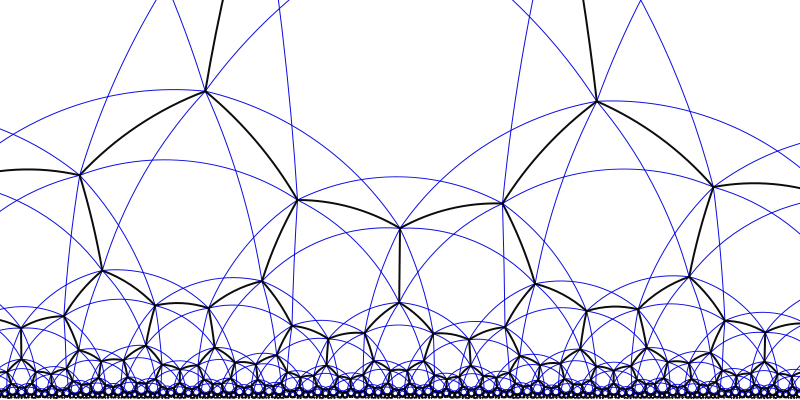
\includegraphics[scale=0.4]{images/hyperbolic_plane.png}
        \end{center}
    \end{figure}
\end{frame}

\begin{frame}{Hiperbolicidad del Plano $\bbm{H}^2$}
    Nuestro objetivo en esta subsección será probar el siguiente resultado:

    \begin{propo}
        El plano hiperbólico $\bbm{H}^2$ (visto como espacio métrico) es un espacio métrico hiperbólico en el sentido de la definición de la sección anterior.
    \end{propo}

    Antes de llegar a ello, probaremos algunos resultados adicionales y enunciaremos algunas definciones.
\end{frame}

\begin{frame}{Hiperbolicidad del Plano $\bbm{H}^2$}
    \begin{mydef}[\textbf{Integral hiperbólica}]
        Sea $\cf{f}{H}{\bbm{R}_\geq0}$ una función Lebesgue integrable. Se define la \textbf{integral de $f$ sobre $\bbm{H}^2$} como:
        \begin{equation*}
            \begin{split}
                \int_{H}f\:dV_H&=\int_{H}f(x,y)\sqrt{\det(G_{H,(x,y)})}\:dxdy\\
                &=\int_{H}\frac{f(x,y)}{y^2}\:dxdy\\
            \end{split}
        \end{equation*}
        donde:
        \begin{equation*}
            G_{ H,(x,y)}=\left(\begin{array}{cc}
                g_{ H,(x,y)}(e_1,e_1) & g_{ H,(x,y)}(e_1,e_2) \\
                g_{ H,(x,y)}(e_2,e_1) & g_{ H,(x,y)}(e_2,e_2) \\
            \end{array} \right)=\left(\begin{array}{cc}
                1/y^2 & 0 \\
                0 & 1/y^2 \\
            \end{array} \right)
        \end{equation*}
        siendo $e_1,e_2\in T_{(x,y)}H=\bbm{R}^2$ los vectores canónicos.
    \end{mydef}
\end{frame}

\begin{frame}{Hiperbolicidad del Plano $\bbm{H}^2$}
    \begin{mydef}[\textbf{Área hiperbólica}]
        Si $A\subseteq H$ es un conjunto Lebesgue medible, definimos el \textbf{área hiperbólica de $A$} por:
        \begin{equation*}
            \mu_{\bbm{H}^2}(A)=\int_{H}\chi_A\:dV_H
        \end{equation*}
        siendo $\chi_A$ la función característica de $A$.
    \end{mydef}
\end{frame}

\begin{frame}{Hiperbolicidad del Plano $\bbm{H}^2$}
    \begin{mydef}[\textbf{Área de un triángulo geodésico}]
        Sea $\Delta$ un triángulo geodésico en $(H,d_H)$. Se define el \textbf{área de $\Delta$} como:
        \begin{equation*}
            \mu_{\bbm{H}^2}(\Delta)=\mu_{\bbm{H}^2}(A_\Delta)
        \end{equation*}
        siendo $A_\Delta\subseteq H$ el conjunto compacto encerrado por las geodésicas de $\Delta$.
    \end{mydef}
\end{frame}

\begin{frame}{Hiperbolicidad del Plano $\bbm{H}^2$}
    \begin{propo}[\textbf{Las isometrías preservan el área}]
        Sea $A\subseteq H$ un conjunto Lebesgue medible y tomemos $f\in\Isom{H,d_H}$. Entonces, $f(A)$ es medible y:
        \begin{equation*}
            \mu_{\bbm{H}^2}(A)=\mu_{\bbm{H}^2}(f(A))
        \end{equation*}
    \end{propo}
\end{frame}

\begin{frame}{Hiperbolicidad del Plano $\bbm{H}^2$}
    \begin{theor}[\textbf{Teorema de Gauß-Bonnet para triángulos hiperbólicos}]
        Sea $\Delta$ un triángulo geodésico en $(H,d_H)$ con ángulos $\alpha,\beta,\gamma$ y suponga que la imagen de $\Delta$ no está contenida en una sola línea geodésica. Entonces:
        \begin{equation*}
            \mu_{\bbm{H}^2}(\Delta)=\pi-(\alpha+\beta+\gamma)
        \end{equation*}
        En particular, la suma de los ángulos de un triángulo geodésico es menor que $\pi$ y el área hiperbólica está acotada por $\pi$.
    \end{theor}
\end{frame}

\begin{frame}{Hiperbolicidad del Plano $\bbm{H}^2$}
    \begin{propo}[\textbf{Crecimiento exponencial del área hiperbólica}]
        Para todo $r\in\bbm{R}_{>10}$ tenemos que:
        \begin{equation*}
            \mu_{\bbm{H}^2}(B_r^{(H,d_H)}(i))\geq e^{\frac{r}{10}}(1-e^{-\frac{r}{2}})
        \end{equation*}
    \end{propo}
    \begin{proof}
        Sea $r\in\bbm{R}_{>10}$. Se tiene que el conjunto:
        \begin{equation*}
            Q_r=\left\{x+iy\Big|x\in[0,e^{ r/10}],y\in[1,e^{r/2}] \right\}
        \end{equation*}
        está contenido en $B_r^{(H,d_H)}(i)$. En particular, obtenemos que:
        \begin{equation*}
            \begin{split}
                \mu_{\bbm{H}^2}(B_r^{(H,d_H)}(i))&\geq\mu_{\bbm{H}^2}(Q_r)\\
                &=\int_{0}^{e^{r/10}}\int_{1}^{e^{r/2}}\frac{dxdy}{y^2}\\
                =&e^{\frac{r}{10}}(1-e^{-\frac{r}{2}})\\
            \end{split}
        \end{equation*}
    \end{proof}
\end{frame}

\begin{frame}{Hiperbolicidad del Plano $\bbm{H}^2$}
    \begin{theor}[\textbf{Triángulos son delgados}]
        Existe una constante $C\in\bbm{R}_{\geq0}$ tal que todo triángulo geodésico en $(H,d_H)$ es $C$-delgado.
    \end{theor}

    \textit{Demostración:}

    Por la proposición anterior, existe $C>0$ tal que:
    \begin{equation*}
        \mu_{\bbm{H}^2}(B_C^{(H,d_H)}(i))\geq 4\cdot\pi
    \end{equation*}
    (por ejemplo $C=26$). Tomemos $\Delta=(\gamma_0,\gamma_1,\gamma_2)$ un triángulo geodésico en $(H,d_H)$ y sea $x\in\im{\gamma_0}$.

    Sin pérdida de generalidad, podemos suponer que el triángulo geodésico $\Delta$ no está contenido en una sola línea geodésica. Por una proposición se sigue que podemos trasladar los puntos $x$ a $i$ y un extremo de la geodésica que lo contiene a un punto tal que:
    %Analizar casos y existencia de transformación de Möbius que manda al 0, 1 y infty
    \begin{equation*}
        \Im f_A(z)>1
    \end{equation*}
    y $\Re f_A(z)=0$.
\end{frame}

\begin{frame}{Hiperbolicidad del Plano $\bbm{H}^2$}
    \begin{figure}
        \begin{center}
            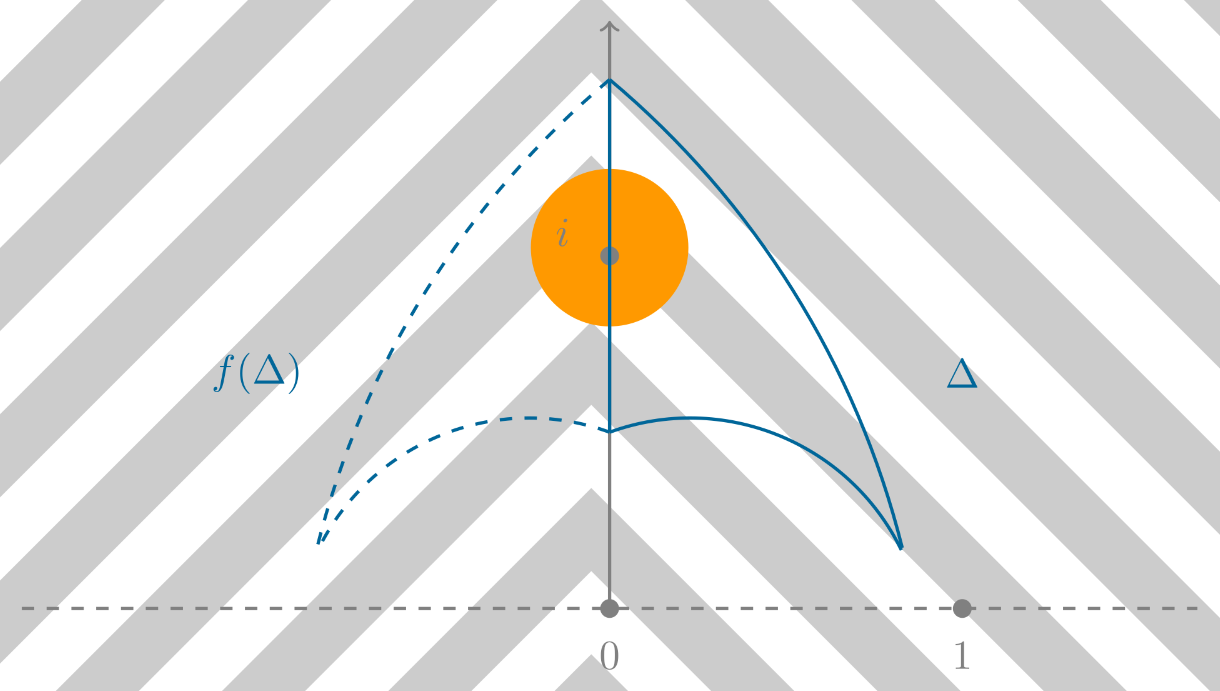
\includegraphics[scale=0.25]{images/hyperbolic_plane_geo_triangle.png}
        \end{center}
        \caption{Movimiento del triángulo $\Delta$.}
    \end{figure}
\end{frame}

\begin{frame}{Hiperbolicidad del Plano $\bbm{H}^2$}
    Luego, de un teorema y otra prosición se sigue que la geodésica $\gamma_0$ es un segmento vertical que yace sobre el eje $y$.

    Supongamos que para todo $y\in\im{\gamma_1}\cup\im{\gamma_2}$ se tiene $d_H(i,y)>C$. Se tiene entonces que:
    \begin{equation*}
        B_c^{(H,d_H)}(i)\subseteq A_\Delta\cup\im{\gamma_0}\cup f(A_\Delta)
    \end{equation*}
    siendo $A_\Delta$ el conjunto encerrado por las geodésicas de $\Delta$ y $\cf{f}{H}{H}$ la isometría $z\mapsto-\overline{z}$.

    %TODO Incluir imagen de qué está pasando.

    Por tanto:
    \begin{equation*}
        \begin{split}
            4\cdot\pi&\leq\mu_{\bbm{H}^2}(B_C^{(H,d_H)}(i))\\
            &\leq\mu_{\bbm{H}^2}(A_\Delta\cup\im{\gamma_0}\cup f(A_\Delta))\\
            &=\mu_{\bbm{H}^2}(A_\Delta)+\mu_{\bbm{H}^2}(\im{\gamma_0})+\mu_{\bbm{H}^2}(f(A_\Delta))\\
            &=\mu_{\bbm{H}^2}(\Delta)+\mu_{\bbm{H}^2}(D)\\
            &< 2\cdot\pi\\
        \end{split}
    \end{equation*}
\end{frame}

\begin{frame}{Hiperbolicidad del Plano $\bbm{H}^2$}
    Lo cual es una contradicción. Por lo cual existe $y\in\im{\gamma_1}\cup\im{\gamma_2}$ tal que $d(x,y)\leq C$. En particular se sigue que:
    \begin{equation*}
        \im{y_0}\subseteq \bigcup_{y\in\im{\gamma_1}\cup\im{\gamma_2}}B_C^{(H,d_H)}(y)\subseteq B_C^{(H,d_H)}( \im{\gamma_1}\cup\im{\gamma_2} )
    \end{equation*}
    el procedimiento anterior se puede repetir para las otras geodésicas, resultando en que:
    \begin{equation*}
        \begin{split}
            \im{\gamma_0}&\subseteq B_{C}^{(H,d_H)}(\im{\gamma_1}\cup\im{\gamma_2}),\\
            \im{\gamma_1}&\subseteq B_{C}^{(H,d_H)}(\im{\gamma_0}\cup\im{\gamma_2}),\\
            \im{\gamma_2}&\subseteq B_{C}^{(H,d_H)}(\im{\gamma_0}\cup\im{\gamma_1})\\
        \end{split}
    \end{equation*}
    así que $\Delta$ es un triángulo geodésico $C$-delgado. Como el $\Delta$ triángulo geodésico fue arbitrario se sigue que el plano hiperbólico es $C$-hiperbólico, es decir que es hiperbólico en el sentido de espacio métrico.
\end{frame}

\begin{frame}{Hiperbolicidad del Plano $\bbm{H}^2$}
    Un resultado más general nos dice lo siguiente:
    \pause
    \begin{theor}[\textbf{Hiperbolicidad de variedades Riemannianias}]
        Si $M$ es una variedad de Riemann cerrada, conexa y de curvatura seccional negativa, entonces el cubriente universal de $M$ es hiperbólico como espacio métrico.
    \end{theor}

\end{frame}

\begin{frame}{Hiperbolicidad del Plano $\bbm{H}^2$}
    \begin{center}
        \Large\textit{Y, ¿para qué nos sirve la hiperbolicidad?}
    \end{center}
\end{frame}

\subsection{Hiperbolicidad es invariante cuasi-isométrico}

\begin{frame}
    \begin{center}
        \Large La hiperbolicidad es un invariante cuasi-isométrico
    \end{center}
\end{frame}

\begin{frame}{Hiperbolicidad es invariante cuasi-isométrico}
    Para llegar a probar tal cosa, debemos debilitar la definición de hiperbolicidad:
    
    \begin{mydef}[\textbf{Triángulos cuasi-geodésicos $\delta$-delgados}]
        Sea $(X,d)$ un espacio métrico.
        \begin{enumerate}[label = \textit{\arabic*}]
            \item Un \textbf{triángulo cuasi-geodésico en $X$} es una tripleta $(\gamma_0,\gamma_1,\gamma_2)$ de $(c,b)-$cuasi-geodésicas $\cf{\gamma_i}{[0,L_i]}{X}$ en $X$ tales que:
            \begin{equation*}
                \gamma_0(L_0)=\gamma_1(0),\quad \gamma_1(L_1)=\gamma_2(0),\quad \gamma_2(L_2)=\gamma_0(0)
            \end{equation*}
            \item Un triángulo $(c,b)$-cuasi-geodésico es \textbf{$\delta$-delgado} si:
            \begin{equation*}
                \begin{split}
                    \im{\gamma_0}&\subseteq B_{\delta}^{(X,d)}(\im{\gamma_1}\cup\im{\gamma_2}),\\
                    \im{\gamma_1}&\subseteq B_{\delta}^{(X,d)}(\im{\gamma_0}\cup\im{\gamma_2}),\\
                    \im{\gamma_2}&\subseteq B_{\delta}^{(X,d)}(\im{\gamma_0}\cup\im{\gamma_1})\\
                \end{split}
            \end{equation*}
        \end{enumerate}
    \end{mydef}
\end{frame}

\begin{frame}{Hiperbolicidad es invariante cuasi-isométrico}
    \begin{figure}
        \begin{center}
            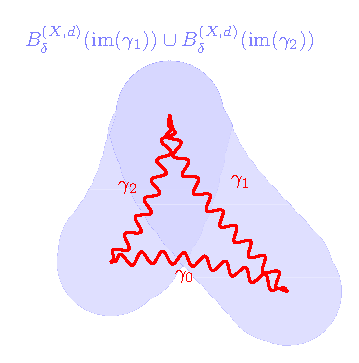
\includegraphics[scale=1.1]{images/delta_slim_qg.pdf}
        \end{center}
        \caption{Triángulo cuasi-geodésico  y $B_\delta^{(X,d)}$}
    \end{figure}
\end{frame}

\begin{frame}{Hiperbolicidad es invariante cuasi-isométrico}
    \begin{center}
        \Large \textit{¿El triángulo $(c,b)$-cuasi-geodésico anterior es $\delta$-delgado?}
        \pause
        
        Sí
    \end{center}    
\end{frame}

\begin{frame}{Hiperbolicidad es invariante cuasi-isométrico}
    \begin{obs}
        De la definición anterior es inmediato que todo triángulo geodésico es triángulo cuasi-geodésico.
    \end{obs}
\end{frame}

\begin{frame}{Hiperbolicidad es invariante cuasi-isométrico}
    \begin{mydef}[\textbf{Espacios cuasi-hiperbólicos}]
        Sea $(X,d)$ un espacio métrico.
        \begin{enumerate}[label = \textit{(\arabic*)}]
            \item Sean $c,b\in\bbm{R}_{>0}$, $\delta\in\bbm{R}_{\geq0}$. Decimos que el espacio $(X,d)$ es \textbf{$(c,b,\delta)$-cuasi-hiperbólico} si $(X,d)$ es $(c,b)$-cuasi-geodésico y todos los triángulos $(c,b)$-cuasi-geodésicos en $X$ son $\delta$-delgados.
            \item Sean $c,b\in\bbm{R}_{>0}$. El espacio $(X,d)$ es llamado \textbf{$(c,b)$-cuasi-hiperbólico} si para todo $c',b'\in\bbm{R}_{>0}$ con $c'\geq c$ y $b'\geq b$ existe $\delta\in\bbm{R}_{\geq0}$ tal que $(X,d)$ es $(c',b',\delta)$-cuasi-hiperbólico.
            \item El espacio $(X,d)$ es \textbf{cuasi-hiperbólico} si existen $c,b\in\bbm{R}_{>0}$ tales que $(X,d)$ es $(c,b)$-cuasi-hiperbólico.
        \end{enumerate}
    \end{mydef}
\end{frame}

\begin{frame}{Hiperbolicidad es invariante cuasi-isométrico}
    \begin{exa}
        Todos los espacios métricos de diámetro finito son cuasi-hiperbólicos.
    \end{exa}

    \begin{obs}
        En general resultará muy complicado probar que un espacio es cuasi-hiperbólico usando la definición anterior, por el hecho de que pueden existir demasiadas cuasi-geodésicas. Resulta que este proceso se puede hacer más sencillo usando unos resultados que se verán más adelante.
    \end{obs}
\end{frame}

\begin{frame}{Hiperbolicidad es invariante cuasi-isométrico}
    \begin{propo}[\textbf{Invariancia de la cuasi-hiperbolicidad bajo cuasi-isometrías}]
        Sean $(X,d)$ y $(Y,\rho)$ espacios métricos.
        \begin{enumerate}[label = \textit{(\arabic*)}]
            \item Si $(Y,\rho)$ es cuasi-geodésico y, $(X,d)$ y $(Y,\rho)$ son cuasi-isométricos, entonces $(X,d)$ es cuasi-geodésico.
            \item Si $(Y,\rho)$ es cuasi-hiperbólico, $(X,d)$ es cuasi-geodésico y existe un encaje cuasi-isométrico de $(X,d)$ en $(Y,\rho)$, entonces $(X,d)$ es cuasi-hiperbólico.
            \item Si $(X,d)$ y $(Y,\rho)$ son cuasi-isométricos, entonces $X$ es cuasi-hiperbólico si y sólo si $Y$ es cuasi-hiperbólico.
        \end{enumerate}
    \end{propo}
\end{frame}

\begin{frame}{Hiperbolicidad es invariante cuasi-isométrico}
    Resulta que no existe mucha diferencia entre la propiedad de hiperbolicidad y cuasi-hiperbolicidad, como lo muestra el siguiente resultado:
    
    \pause

    \begin{theor}[\textbf{Hiperbolicidad y cuasi-hiperbolicidad}]
        Sea $(X,d)$ un espacio métrico geodésico. Entonces $(X,d)$ es hiperbólico si y sólo si es cuasi-hiperbólico.
    \end{theor}

    \pause

    Si $(X,d)$ es cuasi-hiperbólico, entonces es hiperbólico (ya que en particular toda geodésica es una cuasi-geodésica y por ende, todo triángulo geodésico es cuasi-geodésico).

\end{frame}

\begin{frame}{Hiperbolicidad es invariante cuasi-isométrico}
    La idea para probar la otra parte de la demostración de este teorema radica en ver como podemos aproximar cuasi-geodésicas con geodésicas y por ende, aproximar cuasi-triángulos geodésicos con triángulos geodésicos.

    
    \begin{figure}
        \begin{center}
            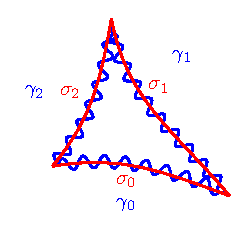
\includegraphics[scale=1.2]{images/approx_geo_cuasi.pdf}
        \end{center}
        \caption{Aproximación del triángulo cuasi-geodésico $\Delta=(\gamma_0,\gamma_1,\gamma_2)$ por el triángulo geodésico $\Delta'=(\sigma_0,\sigma_1,\sigma_2)$.}
    \end{figure}

\end{frame}

\begin{frame}{Hiperbolicidad es invariante cuasi-isométrico}
    \begin{cor}[\textbf{Invariancia cuasi-isométrica de la hiperbolicidad}]
        Sean $(X,d)$ y $(Y,\rho)$ espacios métricos.
        \begin{enumerate}[label = \textit{(\arabic*)}]
            \item Si $(Y,\rho)$ es hiperbólico, $(X,d)$ es cuasi-geodésico y existe un encaje cuasi-isométrico de $(X,d)$ en $(Y,\rho)$, entonces $X$ es cuasi-hiperbólico.
            \item Si $(Y,\rho)$ es geodésico y $(X,d)$ es cuasi-isométrico a $(Y,\rho)$, entonces $(X,d)$ es cuasi-hiperbólico si y sólo si $(Y,\rho)$ es hiperbólico.
            \item Si $(X,d)$ y $(Y,\rho)$ son geodésicos y cuasi-isométricos, entonces $(X,d)$ es hiperbólico si y sólo si $(Y,\rho)$ es hiperbólico. 
        \end{enumerate}
    \end{cor}
\end{frame}

\begin{frame}{Hiperbolicidad es invariante cuasi-isométrico}
    Como algunos ejemplos de la aplicación del teorema anterior tenemos los siguientes:

    \begin{cor}[\textbf{Hiperbolicidad de gráficas}]
        Sea $X$ una gráfica conexa. Entonces $X$ es cuasi-hiperbólica si y sólo si su realización geométrica $\abs{X}$ es hiperbólica.
    \end{cor}

\end{frame}

\begin{frame}{Hiperbolicidad es invariante cuasi-isométrico}
    \begin{propo}[\textbf{Hiperbolicidad de árboles}]
        Si $T$ es un árbol, entonces su realización geométrica $\abs{T}$ es $0$-hiperbólica. En particular, $T$ es cuasi-hiperbólico.
    \end{propo}
\end{frame}

\begin{frame}{Hiperbolicidad es invariante cuasi-isométrico}
    \begin{center}
        \Large\textit{¿Y PARA QUÉ SIRVE LA HIPERBOLICIDAD?}
    \end{center}
\end{frame}

\subsection{Grupos Hiperbólicos}

\begin{frame}
    \begin{center}
        \Large Grupos Hiperbólicos
    \end{center}
    \begin{figure}
        \begin{center}
            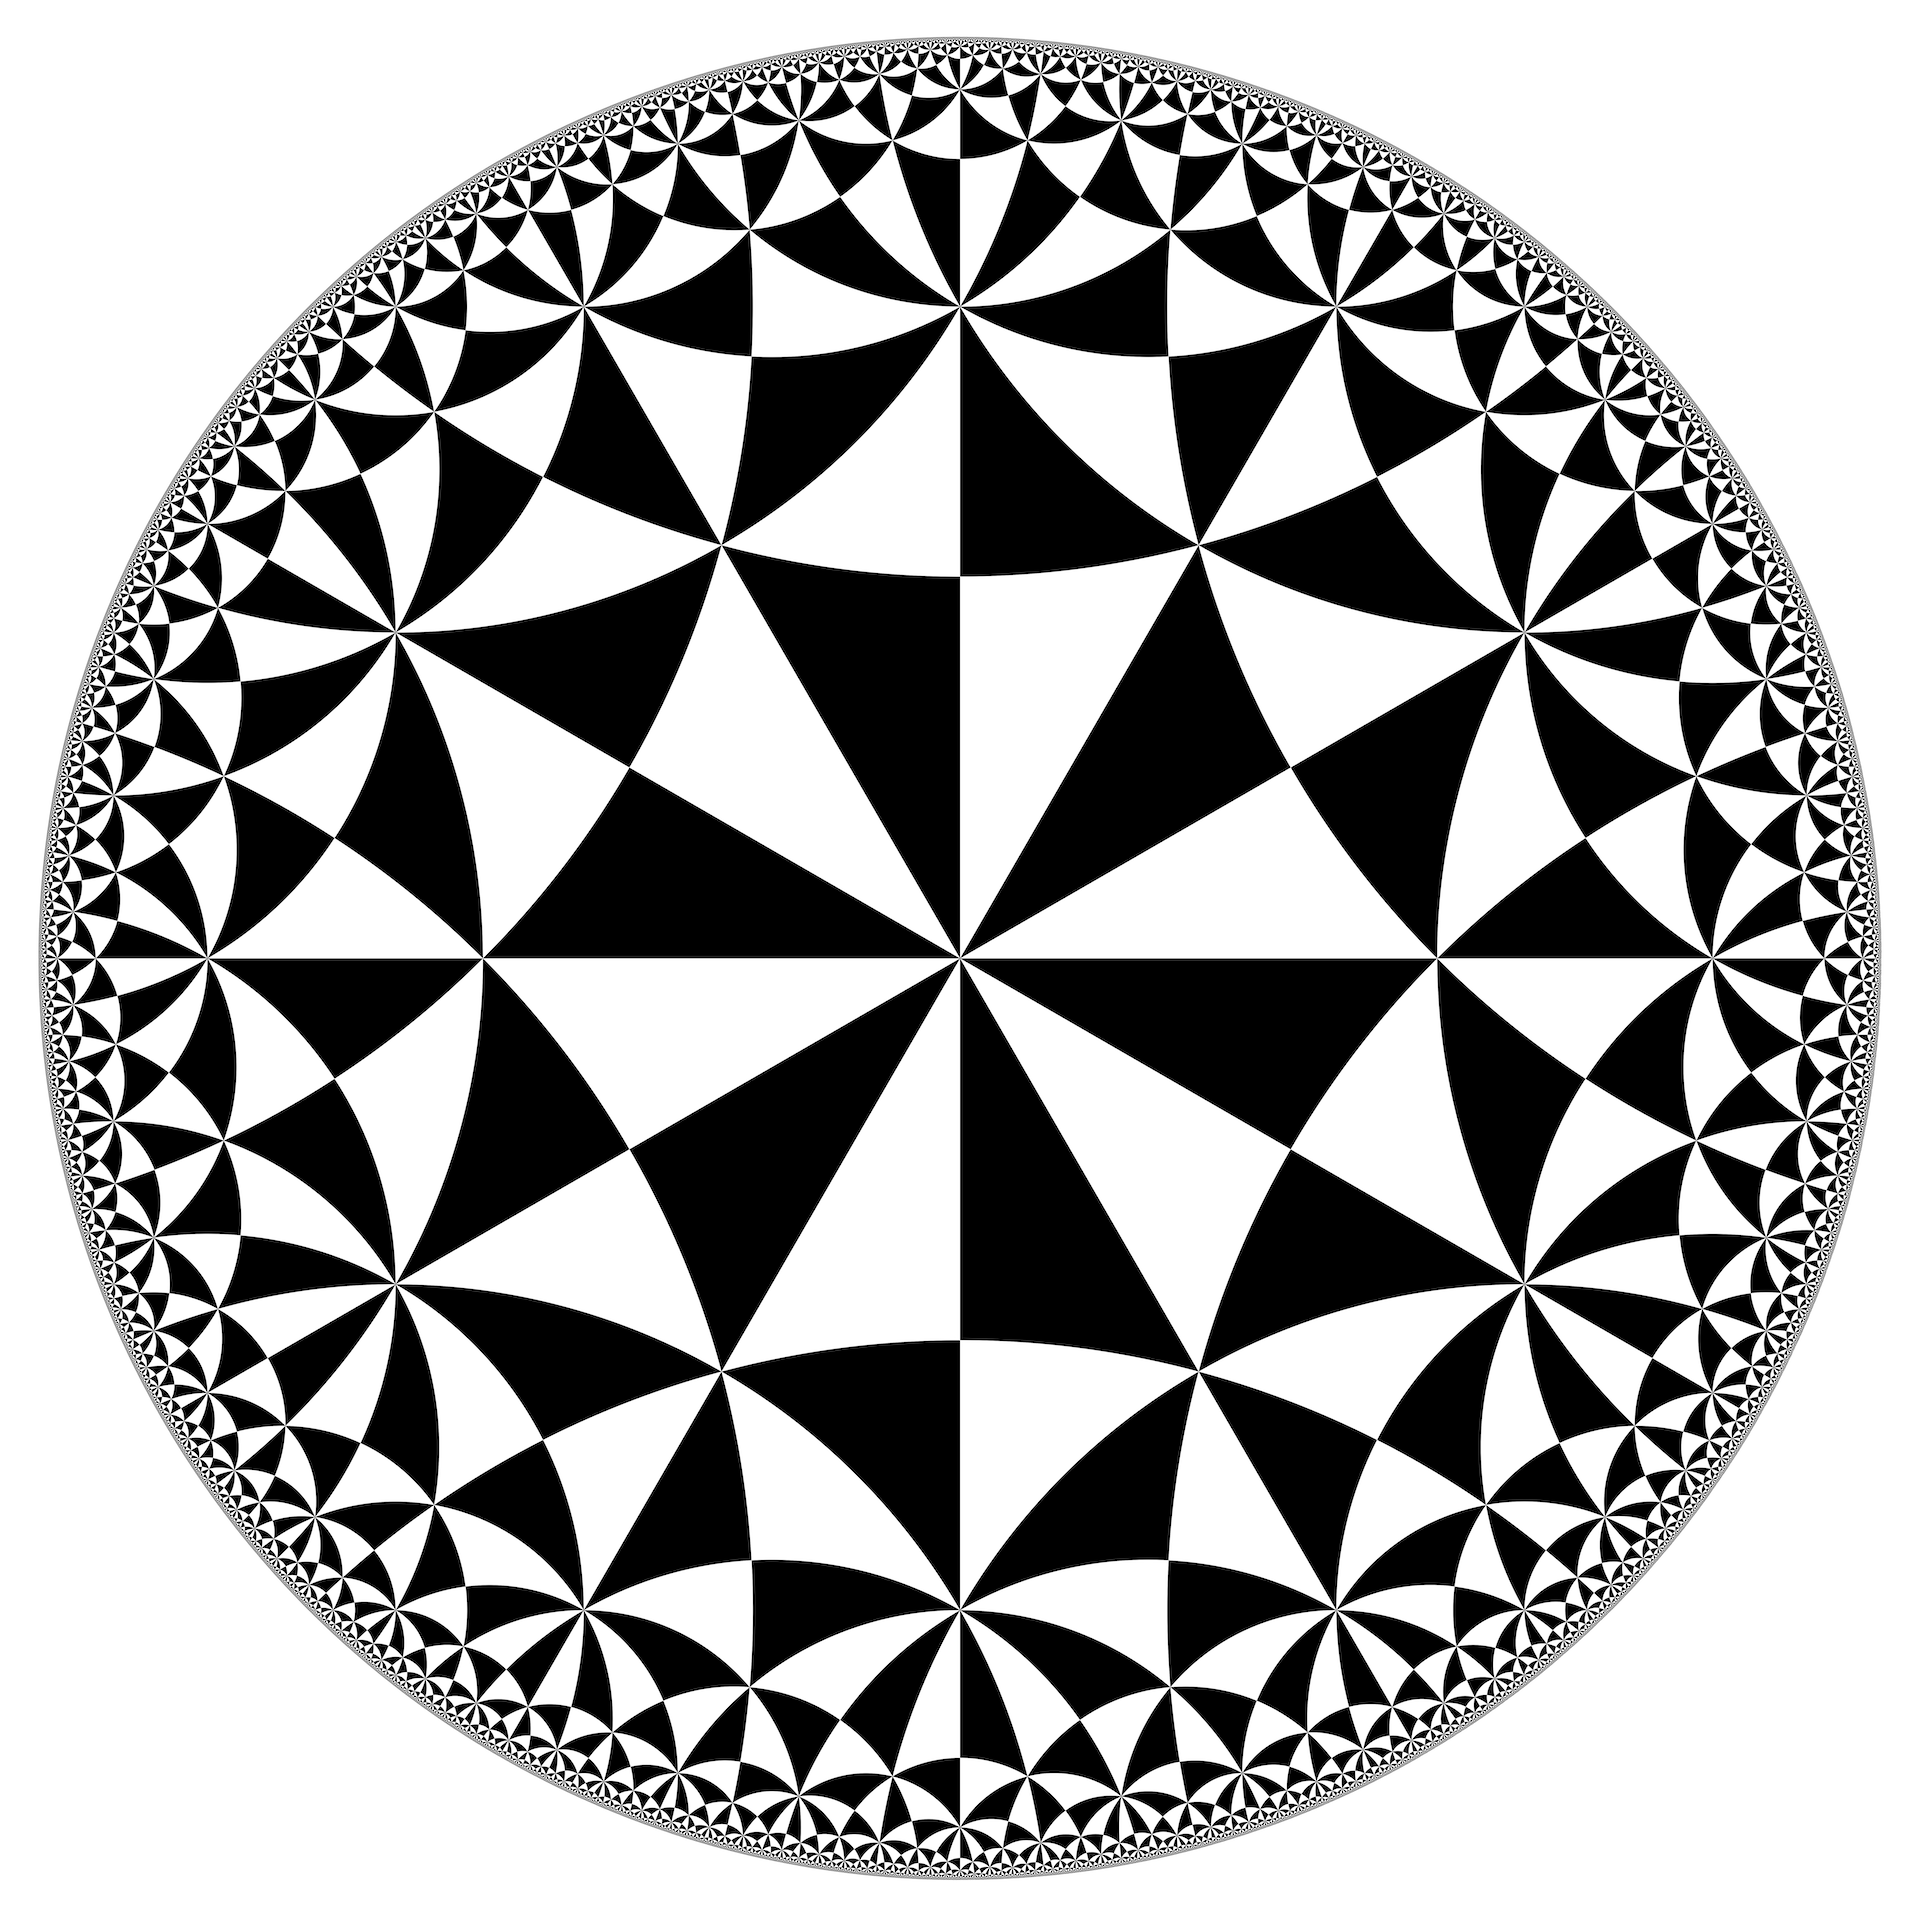
\includegraphics[scale=0.1]{images/disc_tiling.png}
        \end{center}
    \end{figure}
\end{frame}

\begin{frame}{Grupos Hiperbólicos}
    Debido a que la hiperbolicidad (y cuasi-hiperbolicidad) es un invariante cuasi-isométrico, resulta que podemos extender la noción de hiperbolicidad a grupos:

    \begin{mydef}[\textbf{Grupos hiperbólicos}]
        Un grupo finitamente generado $G$ es \textbf{hiperbólico} si para algún conjunto generador $S$ de $G$ se tiene que la gráfica de Caley $\Cay{G,S}$ es cuasi-hiperbólica.
    \end{mydef}
\end{frame}

\begin{frame}{Grupos Hiperbólicos}
    \begin{obs}
        Como la gráfica de Caley de un grupo $G$ es un invariante cuasi-isométrico, es decir que si $S,S'\subseteq G$ son conjuntos finitos que generan a $G$, se tiene que:
        \begin{equation*}
            \Cay{G,S}\qisom\Cay{G,S'}
        \end{equation*}
    \end{obs}
\end{frame}

\begin{frame}{Grupos Hiperbólicos}
    \begin{propo}[\textbf{Hiperbolicidad es un invariante cuasi-isométrico}]
        Sean $G$ y $H$ grupos finitamente generados.
        \begin{enumerate}[label = \textit{(\arabic*)}]
            \item Si $H$ es hiperbólico y existen conjuntos finitos generadores $S$ y $T$, de $G$ y $H$, respectivamente tal que existe un encaje cuasi-isométrico entre $(G,d_S)$ y $(H,d_T)$, entonces $G$ es hiperbólico.
            \item Si $G$ y $H$ son cuasi-isométricos, entonces $G$ es hiperbólico si y sólo si $H$ es hiperbólico.
        \end{enumerate}
    \end{propo}
\end{frame}

\begin{frame}{Grupos Hiperbólicos}
    \begin{exa}
        Todos los grupos finitos son hiperbólicos ya que la realización geométrica de su gráfica de Caley es de diámetro finito.
    \end{exa}

    \begin{exa}
        $\bbm{Z}$ es hiperbólico por ser cuasi-isométrico a $\bbm{R}$, que es un espacio métrico hiperbólico.
    \end{exa}
\end{frame}

\begin{frame}{Grupos Hiperbólicos}
    \begin{exa}
        $\bbm{Z}^2$ no es hiperbólico, ya que es cuasi-isométrico al plano euclideano $\bbm{R}^2$, el cual no es hiperbólico.
    \end{exa}
\end{frame}

\begin{frame}{Grupos Hiperbólicos}
    \begin{center}
        \Large \textit{¿De qué nos sirve generalizar esta noción a grupos?}
    \end{center}
\end{frame}

\subsection{El problema de la palabra en Grupos Hiperbólicos}

\begin{frame}
    \begin{center}
        \Large El problema de la palabra en Grupos Hiperbólicos
    \end{center}

\end{frame}

\begin{frame}{El problema de la palabra en Grupos Hiperbólicos}
    \begin{mydef}
        Sea $\gen{S|R}$ una presentación finita de un grupo. Decimos que \textbf{el problema de la palabra es soluble para la presentación $\gen{S|R}$}, si existe una función total computable que recibe como entrada una palabra en $(S\cup S^{-1})^{*}$ que decida si esta representa o no un elemento trivial en el grupo $\gen{S|R}$.
    \end{mydef}
\end{frame}

\begin{frame}{El problema de la palabra en Grupos Hiperbólicos}
    Al decir que exista una función total computable, en términos más simples estamos diciendo que existe un algoritmo que para cada entrada que demos, termina en un tiempo finito.

    \begin{obs}
        Otra forma de enunciar la definición anterior es que los conjuntos:
        \begin{equation*}
            \begin{split}
                &\left\{w\in(S\cup S^{-1})^*\Big|w\textup{ representa un elemento trivial de }\gen{S|R} \right\}\\
                &\left\{w\in(S\cup S^{-1})^*\Big|w\textup{ no representa un elemento trivial de }\gen{S|R} \right\}\\
            \end{split}
        \end{equation*}
        son conjuntos computablemente enumerables.
    \end{obs}
\end{frame}

\begin{frame}{El problema de la palabra en Grupos Hiperbólicos}
    Al decir que son computablemente enumerables, intuitivamente estamos diciendo que existe un algoritmo que va arrojando todos los elementos de este conjunto.

    \begin{exa}
        La presentación $\gen{x,y|\emptyset}$ tiene problema de la palabra soluble, al igual que $\gen{x,y|xyx^{-1}y^{-1}}$.
    \end{exa}
\end{frame}

\begin{frame}{El problema de la palabra en Grupos Hiperbólicos}
    A primera vista uno podría imaginar que todo grupo finitamente presentado tiene problema de la palabra soluble, cosa que no es cierta, como muestra el siguiente resultado:

    \pause

    \begin{theor}
        Existen grupos finitamente presentados tales que ninguna presentación finita de ellos tiene problema de la palabra soluble.
    \end{theor}
\end{frame}

\begin{frame}{El problema de la palabra en Grupos Hiperbólicos}
    Por ejemplo, se encontró en 1986 que el grupo:
    
    \pause
    
    \begin{figure}
        \begin{center}
            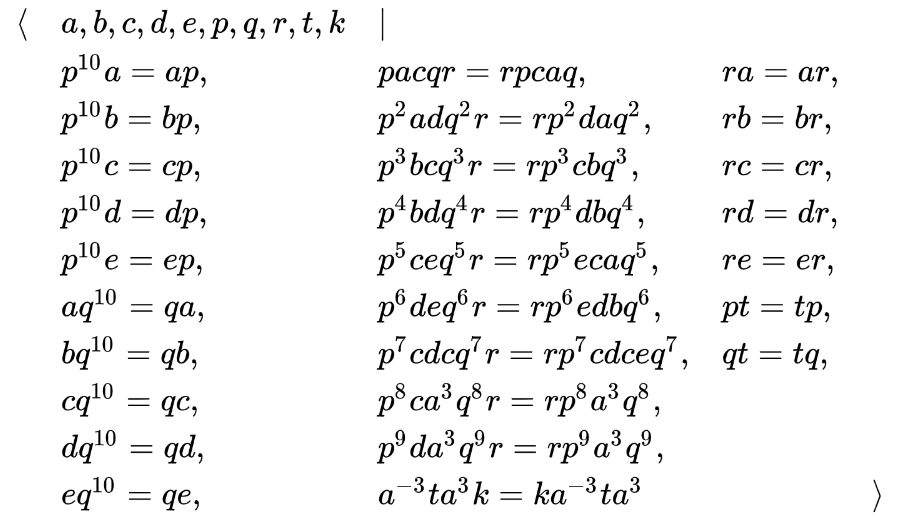
\includegraphics[scale=0.35]{images/no_soluble_word_problem.png}
        \end{center}
    \end{figure}
    
    \pause

    no tiene problema de la palabra soluble.
\end{frame}

\begin{frame}{El problema de la palabra en Grupos Hiperbólicos}
    \begin{mydef}[\textbf{Presentaciones de Dehn}]
        Una presentación finita $\gen{S|R}$ es una \textbf{presentación de Dehn} si existe $n\in\bbm{N}$ y palabras $u_1,...,u_n,v_1,...,v_n$ tales que:
        \begin{itemize}
            \item $R=\left\{u_1v_1^{-1},...,u_nv_n^{-1} \right\}$.
            \item Para todo $j=1,...,n$, la palabra $v_j$ es más corta que $u_j$.
            \item Para topa palabra $w\in(S\cup S^{-1})^*\setminus\left\{e\right\}$ que representa un elemento neutro del grupo $\gen{S|R}$ existe $j=1,...,n$ tal que $u_j$ es subpalabra de $w$.
        \end{itemize}
    \end{mydef}
\end{frame}

\begin{frame}{El problema de la palabra en Grupos Hiperbólicos}
    \begin{exa}
        La presentación:
        \begin{equation*}
            \gen{x,y|xx^{-1}e,yy^{-1}e,x^{-1}xe,y^{-1}ye}
        \end{equation*}
        es una presentacion de Dehn del grupo libre de rango 2.
    \end{exa}

    \pause

    \begin{exa}
        La presentación:
        \begin{equation*}
            \gen{x,y|[x,y]}
        \end{equation*}
        no es una presentación de Dehn de $\bbm{Z}^2$.
    \end{exa}
\end{frame}

\begin{frame}{El problema de la palabra en Grupos Hiperbólicos}
    \begin{propo}[\textbf{Algoritmo de Dehn}]
        Si $\gen{S|R}$ es una presentación de Dehn, entonces el problema de la palabra es soluble para $\gen{S|R}$.
    \end{propo}
    \textit{Demostración}:

    Escribimos:
    \begin{equation*}
        R=\left\{u_1v_1^{-1},...,u_nv_n^{-1} \right\}
    \end{equation*}
    como en la definición de presentación de Dehn. Tomemos $w\in(S\cup S^{-1})^*$ una palabra.
    \begin{itemize}
        \item Si $w=e$, entonces $w$ representa un elemento trivial del grupo $\gen{S|R}$.
        \item Si $w\neq e$, tenemos dos casos:
        \begin{itemize}
            \item Si ninguna de las palabras $u_1,...,u_n$ es una subpalabra de $w$, entonces $w$ no representa un elemento trivial del grupo $\gen{S|R}$ (por la tercera parte de la definción de presentaciones de Dehn).
        \end{itemize}
    \end{itemize}
\end{frame}

\begin{frame}{El problema de la palabra en Grupos Hiperbólicos}
    \begin{proof}
        \begin{itemize}
            \item Si $w\neq e$, tenemos dos casos:
            \begin{itemize}
                \item Existe $j=1,...,n$ tal que $u_j$ es subpalabra de $w$, en cuyo caso se sigue que existen palabras $w',w''$ tales que: $w=w'u_jw''$. Ahora, como $u_jv_j^{-1}\in R$ se sigue que los elementos:
                \begin{equation*}
                    w'u_jw''\quad\textup{y}\quad w'v_jw''
                \end{equation*}
                representan el mismo elemento en el grupo $\gen{S|R}$. Así que la palabra $w$ es trivial si y sólo si la palabra $w'v_jw''$ (que es más corta) es trivial. Aplicando recursivamente el algoritmo se llega a determinar si $w$ es la palabra trivial o no.
            \end{itemize}
        \end{itemize}
        Este algoritmo siempre determina si la palabra $w$ es trivial o no, por lo que el problema de la palabra es soluble en $\gen{S|R}$.
    \end{proof}
\end{frame}

\begin{frame}{El problema de la palabra en Grupos Hiperbólicos}
    \begin{theor}[\textbf{Presentaciones de Dehn en grupos hiperbólicos}]
        Sea $G$ un grupo hiperbólico y $S$ un conjunto generador de $G$. Entonces existe un conjunto finito $R\subseteq(S\cup S^{-1})^*$ tal que $\gen{S|R}$ es una presentación de Dehn y $G\cong\gen{S|R}$.
    \end{theor}
\end{frame}

\begin{frame}{El problema de la palabra en Grupos Hiperbólicos}
    \begin{cor}[\textbf{Grupos hiperbólicos tienen problema de la palabra soluble}]
        Sea $G$ grupo hiperbólico y $S\subseteq G$ un conjunto generador finito. Entonces existe una presentación finita $\gen{S|R}$ de $G$ tal que el problema de la palabra es soluble.
    \end{cor}

    \pause

    \begin{center}
        ¡¡Todo grupo hiperbólico finitamente generado tiene problema de la palabra soluble!!
    \end{center}
\end{frame}

%DAr ejemplos

\begin{frame}
    \Huge{\centerline{\textbf{Fin}}}
\end{frame}

\begin{frame}{Referencias}
    \footnotesize
    \bibliography{reference.bib}
    \bibliographystyle{apalike}
\end{frame}

\end{document}